% COPY AND PASTE THE CODE THROUGH "START YOUR DOCUMENT" FOR EACH NEW REPORT
% - - - - - - - - - - - - - - - - - - - - - - - - - - - - - - - - - - - - - - - - - -
\documentclass[12pt]{article}

% import mathy things
\usepackage{amssymb}
\usepackage{amsmath}
\usepackage{amsthm}
\usepackage{booktabs}
\usepackage{float}
\usepackage[export]{adjustbox}
\newtheoremstyle{exmp}{3pt}{3pt}{\small}{\parindent}{\bfseries}{:}{0.5em}{}
\theoremstyle{exmp}
\newtheorem{example}{Example}

% use pictures and colors
\usepackage{graphicx}
\usepackage[usenames,dvipsnames]{color}
\usepackage{xcolor}

\usepackage[font=scriptsize]{caption}

% set page margins
\usepackage[top=1in, bottom = 0.7in, left=1in, right = 1in,letterpaper]{geometry}

\usepackage{hyperref}
\usepackage{enumerate}
% usepackage{epstopdf} 	%% uncomment to import .eps files on a Mac.
\usepackage{mdwlist}
\usepackage{ulem}
\usepackage{fancyhdr}
\usepackage{lastpage}

%\linespread{1.1}	% slightly more than single-spaced lines

% = = = = = = = = [BEGIN DO_NOT_EDIT]= = = = = = = = = = = = = =
%% Define custom commands for scientific review
%\newcommand\reporttitle[1]{{#1}}
%\newcommand{\reportsubtitle}[1]{{\large Application Excursion \#{#1}}\\[-0.5em]{\normalsize\textsc{Math 295: Computational Modeling}}}
%% setup for title and author(s)
%\makeatletter
%\newcommand{\makeReportTitle}{% 
%\title{\reporttitle \\ \reportsubtitle{\reportnumber}}
%
%  \@ifundefined{authortwo}{%
% 	\author{\authorone}%
%	}{%
%	\@ifundefined{authorthree}{%
%  		\author{\authorone \and \authortwo}%
%		}{%
% 		\author{\authorone \and \authortwo \and \authorthree}%
%		}}%
% 
%\maketitle
%\thispagestyle{empty}
%}
%\makeatother

% customize page numbers -- typeset TWICE to update page reference (eliminates ??)
\pagestyle{empty}
\makeatletter \renewcommand{\@evenhead}{%
%\normalsize\slshape DRAFT \today\hfil \upshape %
\small \texttt{Team \#~1926166 \hfill  {Page~\thepage} of \pageref{LastPage}}} \renewcommand{\@oddhead}{\@evenhead} \makeatother

% - - - - - - - - - - - - - - - - - - - - - - - - - - - - - - - - - - 
% = = = = = = = = [END DO_NOT_EDIT]= = = = = = = = = = = = = = 


















% = = = = = = = = = = = = = = = = = = = = = = = = = = = = = = 
%		SETUP TITLE PAGE -- UPDATE {content} FOR EACH NEW ASSIGNMENT
% = = = = = = = = = = = = = = = = = = = = = = = = = = = = = = 

% DEFINE A DESCRIPTIVE REPORT TITLE GIVEN THE TOPIC OF YOUR REPORT
\title{}
%\author{Team 93321}% per ICM instructions, DO NOT include your names!
\date{}

% = = = = = = = = = [END TITLE PAGE SETUP] = = = = = = = = = = = = 				
% = = = = = = = = = = = = = = = = = = = = = = = = = = = = = = 








% = = = = = = = = = = = = = = = = = = = = = = = = = = = = = = 
%				START YOUR DOCUMENT
% = = = = = = = = = = = = = = = = = = = = = = = = = = = = = = 
\begin{document}		% Text will appear after this command


% make title page - DO NOT EDIT
\makeatletter
%\maketitle
\thispagestyle{fancy} 
\chead{\small \texttt{Team \#~1926166 \hfill  {Page~\thepage} of \pageref{LastPage}}} 
\makeatother
% = = = = = = = = = = = = = = = = = = = = = = = = = = = = = = 

% - - - - - - - - - - - TABLE OF CONTENTS - - - - - - - - - -
\tableofcontents 	% Typeset 2 or 3 times to update page numbers in table of contents

% - - - - - - - - - - - REPORT STARTS HERE - - - - - - - - - -


% - - - - - - - - - - - Introduction - - - - - - - - -
\newpage
\section{Introduction} 
\label{sec:introduction} 
\subsection{Problem Background}
In recent years, the United States is facing a countrywide problem with respect to drug abuse as prescription use and  illicit recreational use. Drug abuse will undermine human health and personal property as using drugs disorderly may cause hepatitis, HIV infection, and also neonatal abstinence syndrome. Federal government and organizations are trying their best to ``save lives and prevent negative health effects of this epidemic''.[1] Thus, for the purpose of countering the opioid crisis, in this paper we will: \begin{itemize}
    \item Use the 2010-2017 NFLIS data provided to model the spread and find the characteristics of the reported synthetic opioids and heroin incidents in and between the five states, Ohio, Kentucky, West Virginia, Virginia, and Pennsylvania in terms of their counties for trend analysis.
    \item Use the U.S Census socio-economic data provided to improve the model we constructed and give a more precise % need to be modified
    \item Identify strategies for countering the opioids crisis.
\end{itemize}


\subsection{Previous Research}
Since this topic involves the interaction between adjacent counties, it is very similar to the model focusing on infectious disease propagation. We looked up for various researches about this topic and found that most of them are based on Cellular Automaton algorithm (CA), such as Yu Lei, Xue Hui-Feng, Gao Xiao-Yan, and Li Gang's research on the transmission of SARS in 2007.[2] The major work that we refer to is Sirakoulis, Karafyllidis, and Thanailakis's research about effects of population on epidemic propogation.[3] %Other works like Steady Mushayabasa's research on illicit drug use in South Africa use his own mathematical model to illustrate the numerical results in 2015.%NEED MORE WORK ON THIS
%The major work that we refer to is the Steady Mushayabasa's research paper and his model.

\subsection{Our work}
In this solution, we first, by referring to Sirakoulis et al's model, build the CA model for the spread of drugs that we can apply data of heroine or synthetic opioid from the year 2010 to 2017 with the provided NFLIS data, analyze patterns and characteristics of the reports, and evaluate the future trends as well as origin locations based upon the model. Then we add the U.S. Census socio-economic data into consideration, by which we find influential factors from the data set that help explain the drug-use trend. For the last part, we would modify the influential factors in the model to determine a possible strategy for countering the opioid crisis.

 % labels allow you to cross-reference a section later in the document, without having to remember its number
%  - - - - - - - - - - - - - - - - - - - - - - - - - - - - - -
% Delete existing text when writing your own report.


 

% - - - - - - - - - - - END Introduction - - - - - - - - - - -


% - - - - - - - - - - - Model Design - - - - - - - - -
\section{Assumptions} 

\begin{itemize}
    \item The NFLIS data and US Socio-economic data are correct as provided.
    
    \item Drug can only be transported from one county to its adjacent counties. 
    
    \item The number of people who stop taking drugs forever after drug treatment is neglected.
    \item The population in each county will remain constant over years. 
    \item People only acquire drugs in the county that they are residing.
    \item In every year, the county which has nonzero drug reports will influence its adjacent counties merely by increasing each one's number of drug reports.
    \item In every year, the number of drug reports in a county will decrease merely because of law enforcement.
    %Since the rate of drug relapse is relatively high (about 85$\%$) within a year after drug treatment action, we assume that once one got addicted to drugs, he or she will constantly be dependent on drugs.[4]
    % remember to reference the 85% data.
    % delete the third one. Conjecture: Since only 85% of addicted people can withdraw, drug reports in each county will keep increasing unless a law enforcement
    
\end{itemize}

%---------------------End Assumption------------------------

\vspace{-.5em}
\begin{table}
\centering
\begin{tabular}{c|l}
\toprule \\
Nomenclature & Meaning \\
\hline
$N(t)$ & total population \\

$S(t)$ & individuals who are not yet illicit drug users but interact with drug users \\

$I(t)$ & light or occasional drug users \\

$I_a(t)$ & heavy drug users \\

$M(t)$ & people who have mentally illness \\

$R(t)$ & detected illicit drug users \\

$\beta$ & strength of intersection between the susceptible individuals and illicit drug users \\

$\kappa$ & \makecell{the modification factor that accounts for the increased likelihood of heavy illicit drug \\ & users to influence more new drug users compared with light drug users} \\

$\alpha$ & the rate at which light drug users become heavy drug users \\

$\gamma$ & rate of detection and rehabilitation of individuals in class $I$ \\

$\epsilon$ & rate of detection and rehabilitation of individuals in class $M$ \\

$\rho$ & rate of detection and rehabilitation of individuals in class $I_a$ \\

$\sigma$ & rate at which light illicit drug users develop mental health \\

$\phi$ & rate at which heavy illicit drug users develop mental health \\

$\psi$ & permanent exit rate of light drug users \\

$d$ & permanent exit rate of heavy drug users \\

$\omega$ & rate at which individuals in rehabilitation recover \\

$\delta$ & rate at which mentally ill individuals permanently exit the model \\
\bottomrule
\end{tabular}
\end{table}
% labels allow you to cross-reference a section later in the document, without having to remember its number
%  - - - - - - - - - - - - - - - - - - - - - - - - - - - - - -
% Delete existing text when writing your own report.

\section{Spread and Characteristics of Synthetic Opioids and Herion Incidents}

In this section, we are going to build a CA model to describe and predict the trends of the drug usage in the five states we are focusing on: Ohio, Kentucky, West Virginia, Virginia, and Pennsylvania. First we categorize the list of narcotic analgesic by synthetic, semi-synthetic, and non-synthetic opioids. Then the list of synthetic opioids contains all drugs other than Buprenorphine, Codeine, Heroin, Hydrocodone, Hydromorphone, Hydorcodeinone, Morphine, Opiate, Opium, Oxycodone, Oxymorphone, and Thebaine.\\
For heroin and synthetic opioids, we make heat maps for the number of drug reports within the five states from 2010 to 2017 respectively.  Using these graphs, we can easily visualize the trends of drug usage and trace its development along the timeline. Then, referring to Sirakoulis et al's work, we construct the corresponding CA model, which can be successfully tested by the given data in eight years. By using this model, we are able to predict the future trend-in-use and, in a reversed direction, locate the starting points of specific opioids in each of five states.  

 
\subsection{Visualization of Drug Reports}
Since the numbers of annual reports about Herion increase at roughly the same rate as year passes during 2010-2013, we only show the distribution of annual reports geographically during 2014-2017, where significant and noteworthy changes occurred. The situation is similar to that of synthetic opioids, so we would also do the same thing to them.\\
In the following graphs, we use different shades of blue colors and orange colors to represent the number of heroin and synthetic opioid reports from the year of 2014 to 2017. The blue colors represent the number of annual Heroin reports in each county and the orange colors represent that of synthetic opioids.  The deeper the color of the county is, the more reports that county had in that year. 
~\\
 As told by the data, the number of annual Heroine reports experienced a mild growth every year. On the other hand, the amount of synthetic opioids reports  experienced a dramatically growth from year 2014 to year 2017, especially in Ohio.  As a result, the pictures we showed are chosen specifically for these changes.

%----------------------------------------------------------------
%----------------------ADD IT BACK!!!----------------------------
%----------------------------------------------------------------

% \begin{figure}[H]
%   \begin{minipage}{0.48\textwidth}
%      \centering
%      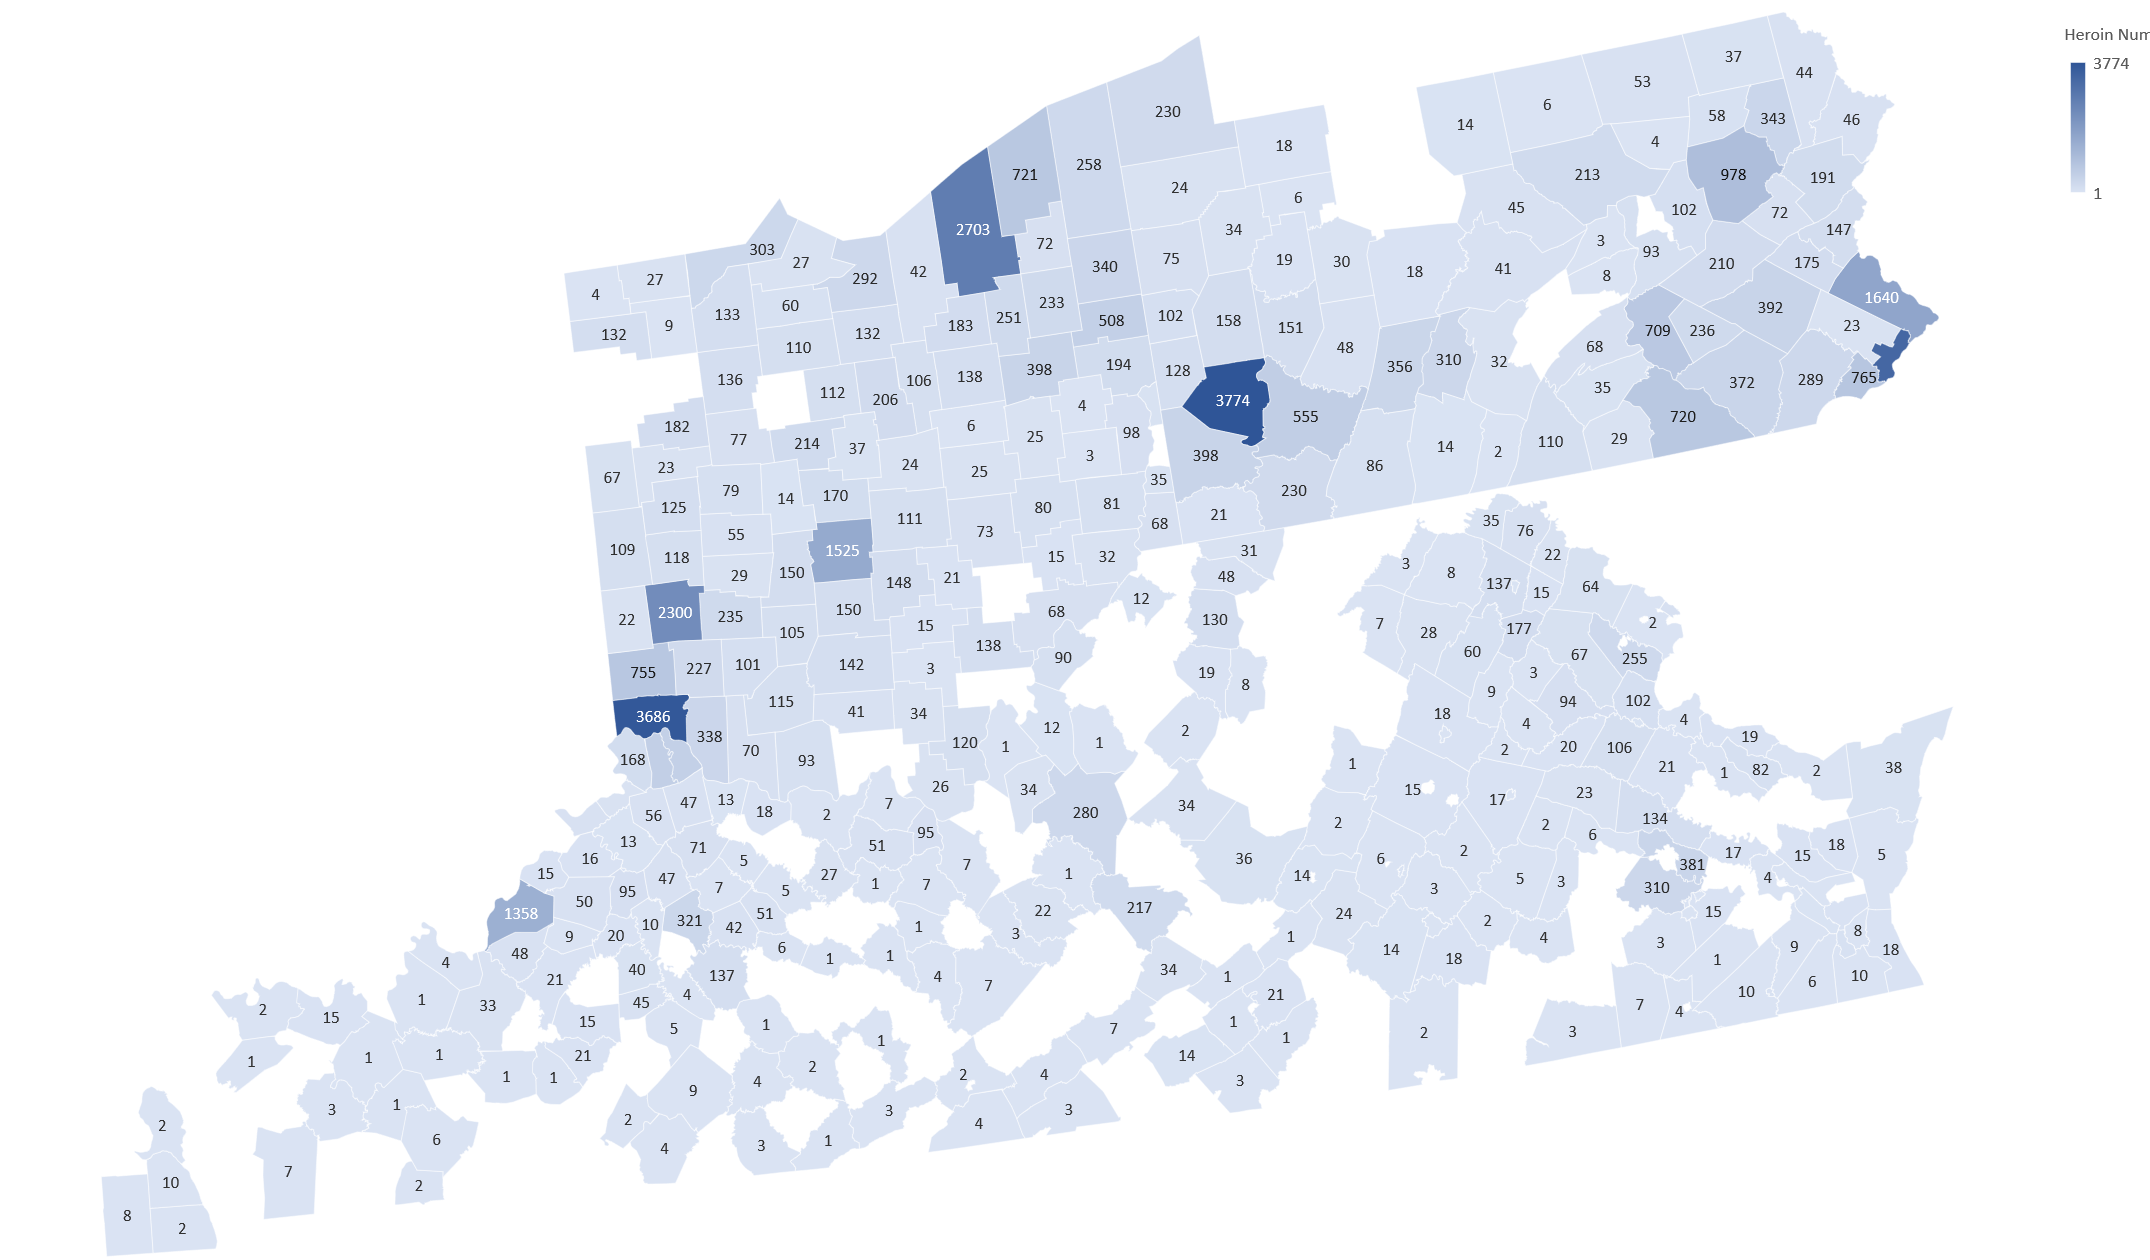
\includegraphics[width=\linewidth]{2014.png}
%      \caption{2014 Heroin}\label{H14}
%   \end{minipage}%\hfill
%   \begin{minipage}{0.48\textwidth}
%      \centering
%      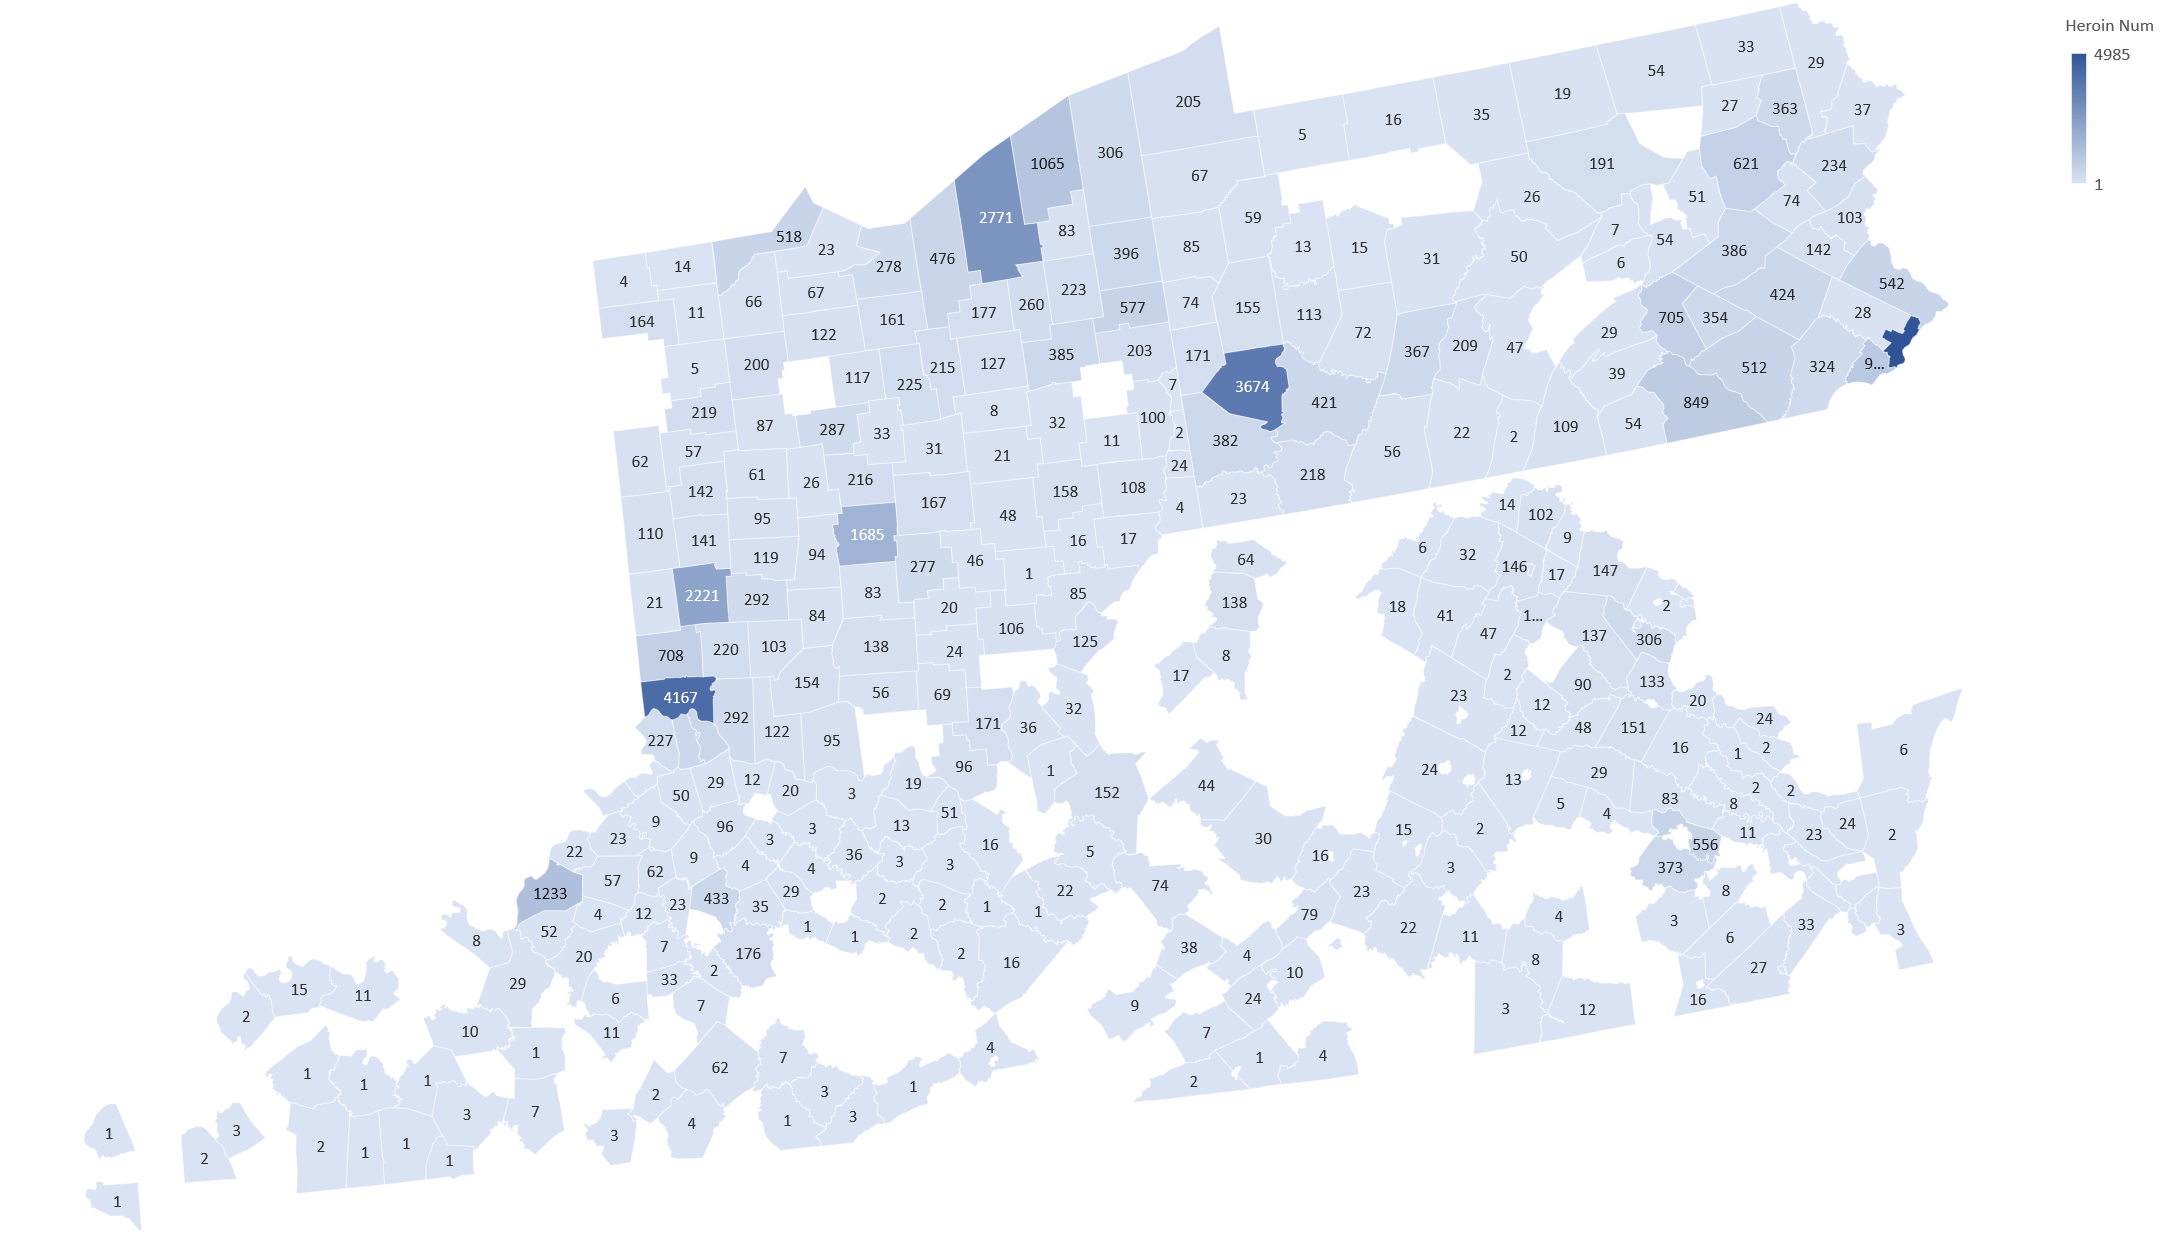
\includegraphics[width=\linewidth]{2015.png}
%      \caption{2015 Heroin}\label{H15}
%   \end{minipage}
% \end{figure}

% \begin{figure}[H]
%   \begin{minipage}{0.5\textwidth}
%      \centering
%      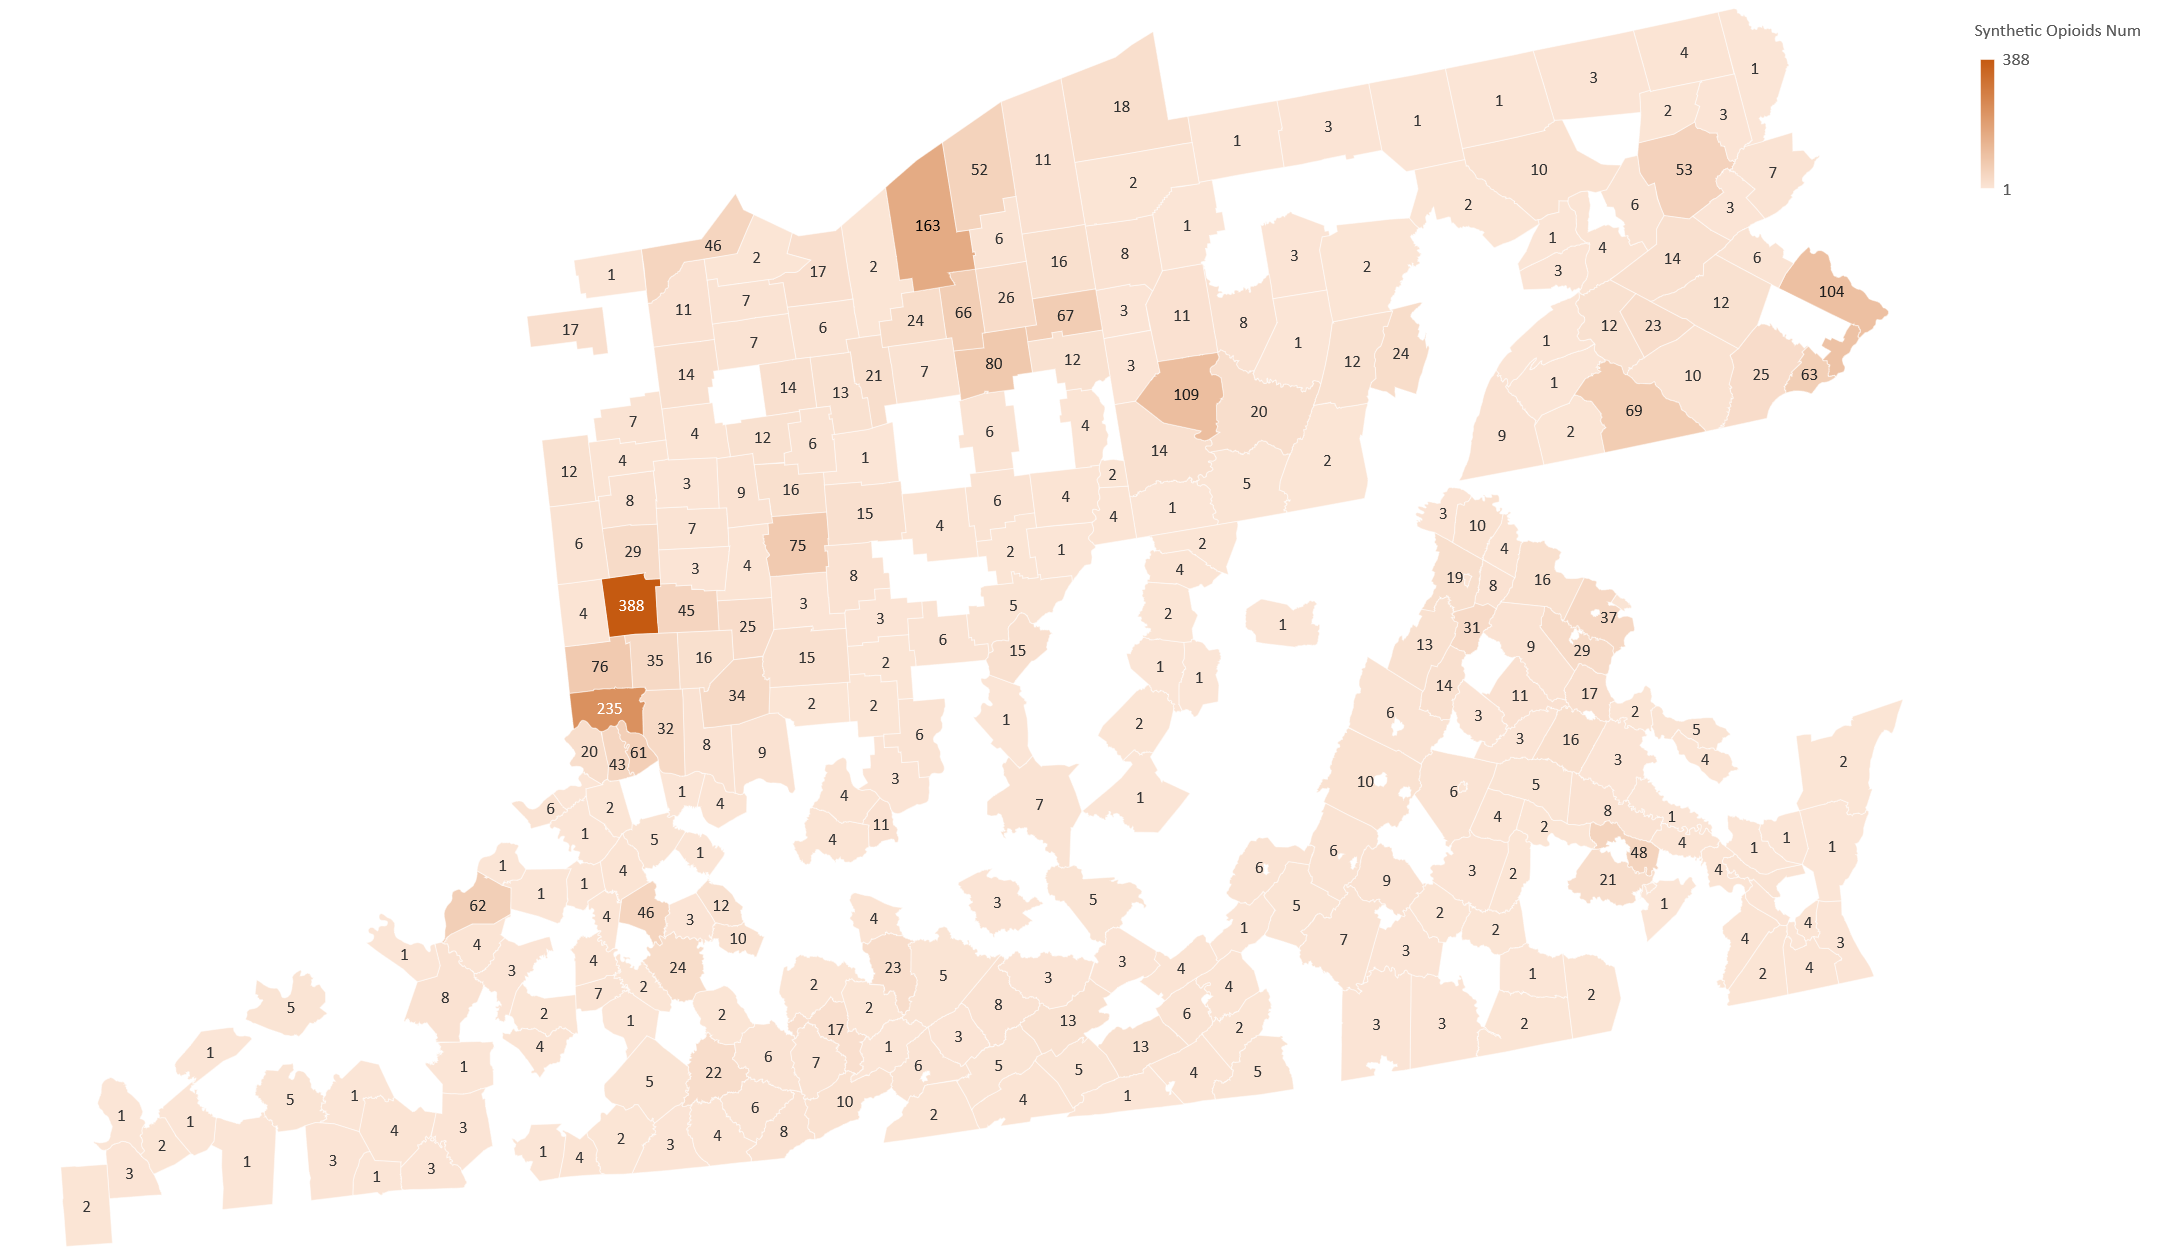
\includegraphics[width=\linewidth]{2014SYN.png}
%      \caption{2014 Synthetic}\label{S14}
%   \end{minipage}%\hfill
%   \begin{minipage}{0.5\textwidth}
%      \centering
%      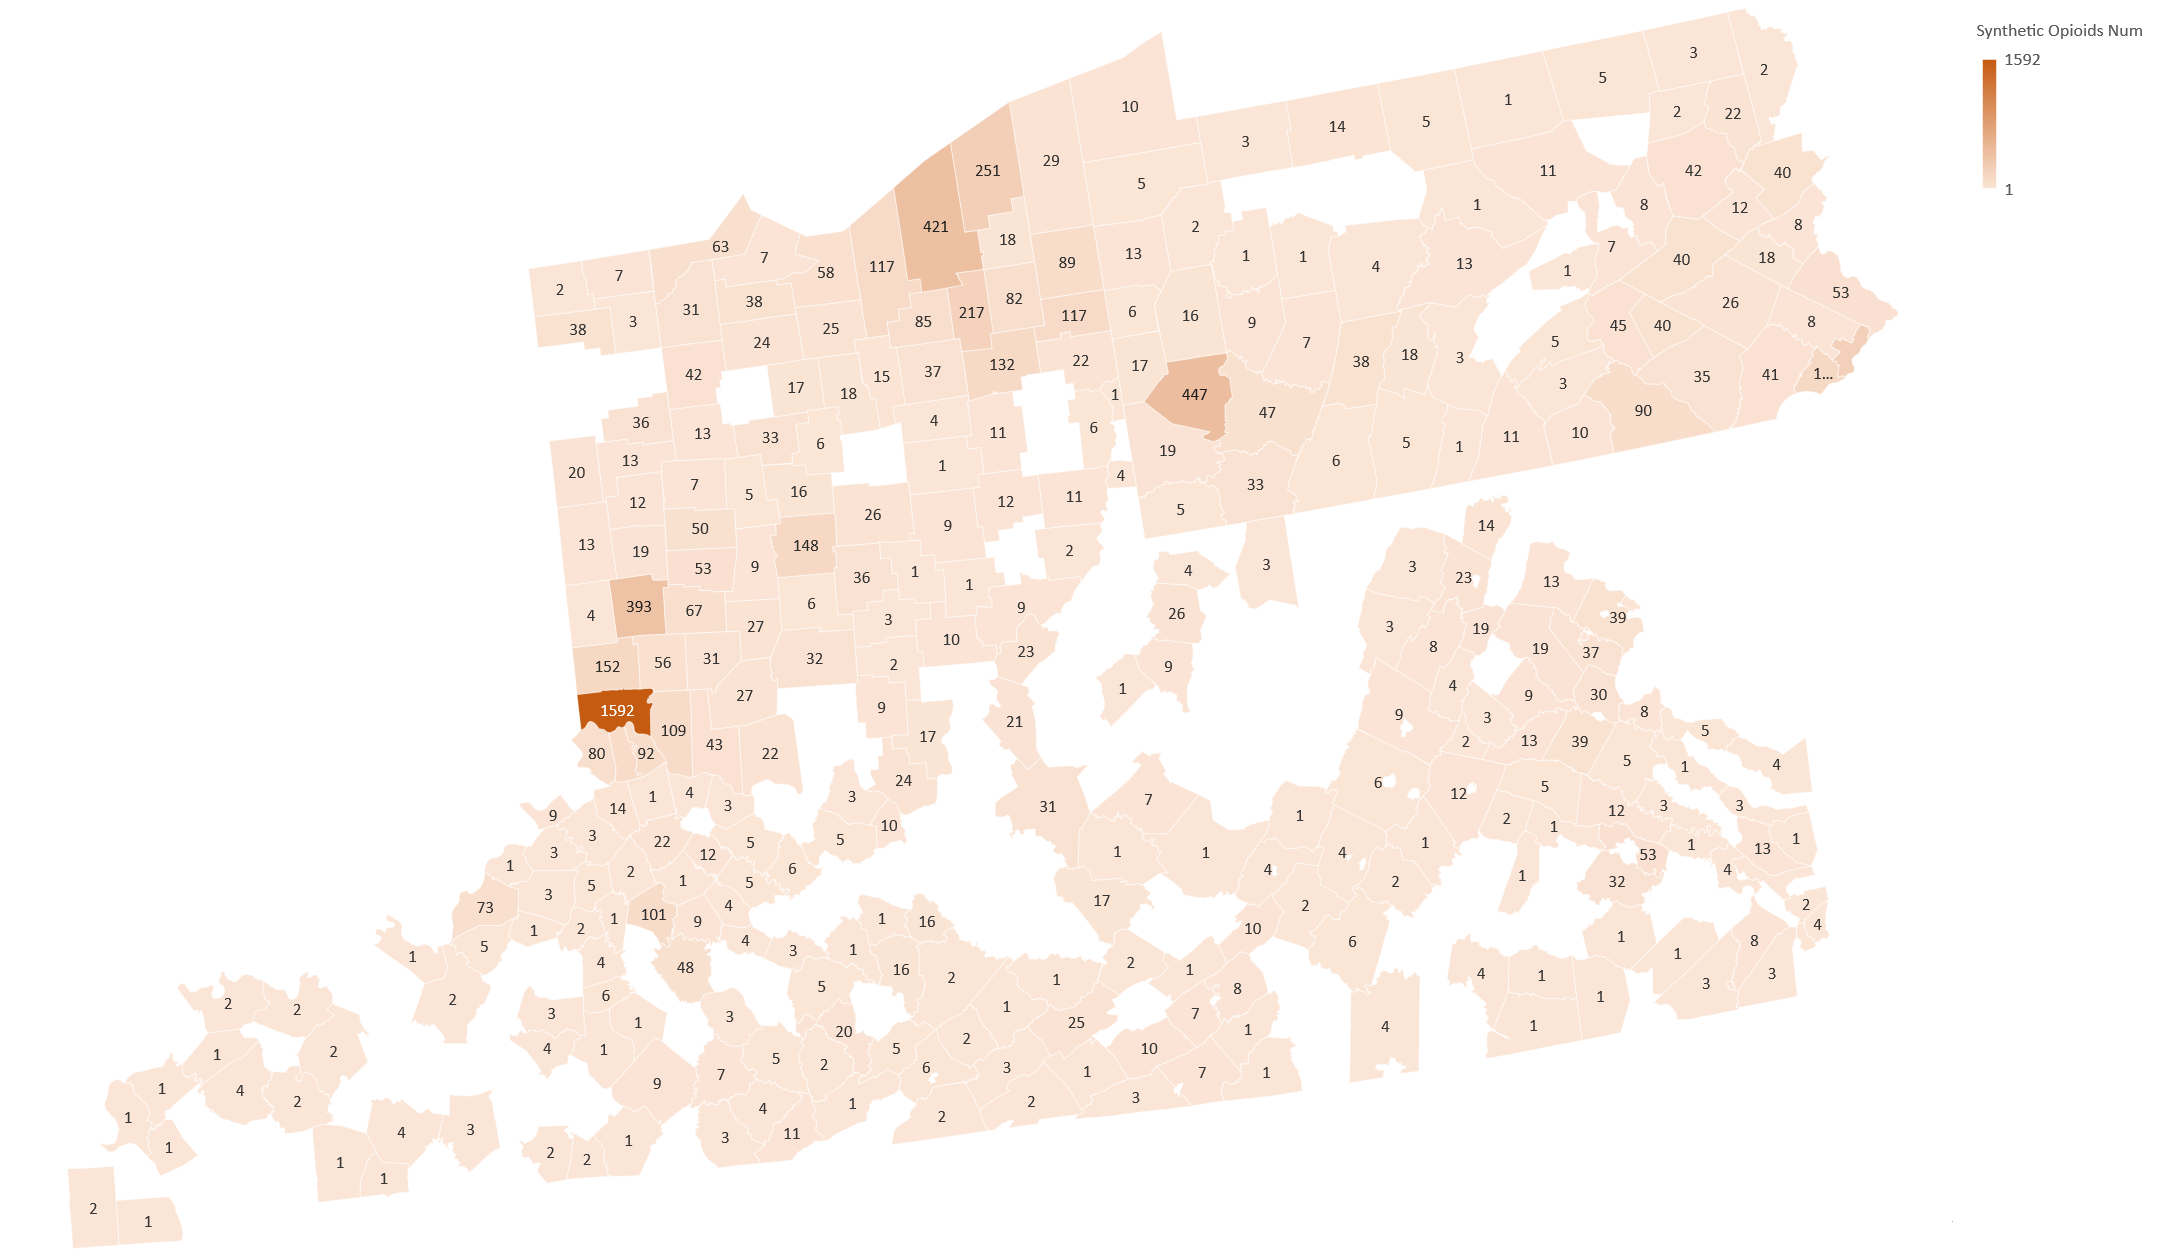
\includegraphics[width=\linewidth]{2015SYN.png}
%      \caption{2015 Synthetic}\label{S15}
%   \end{minipage}
% \end{figure}

% \begin{figure}[H]
%   \begin{minipage}{0.5\textwidth}
%      \centering
%      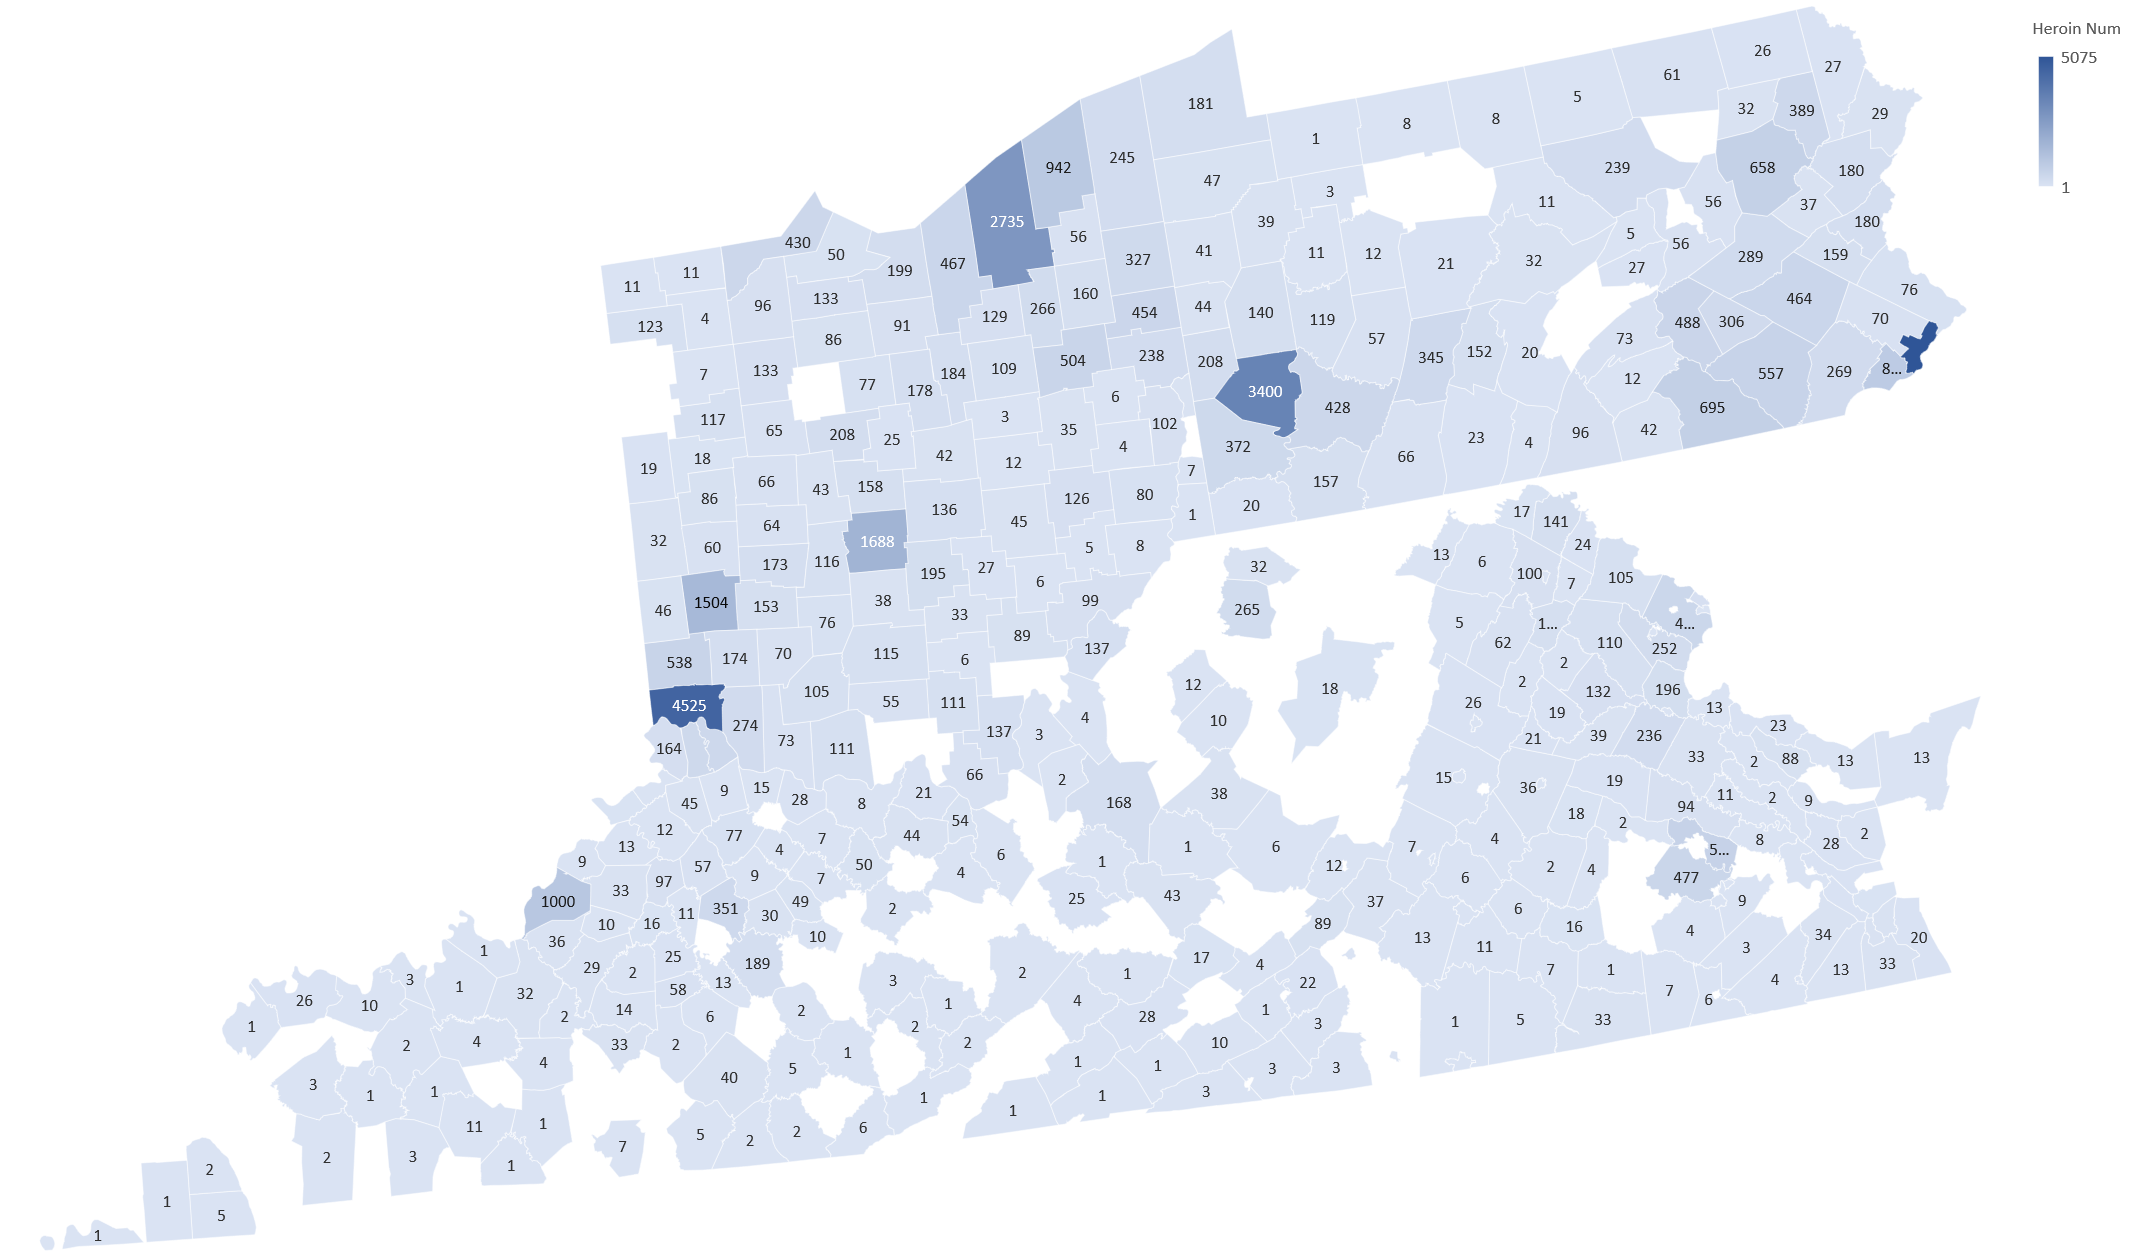
\includegraphics[width=\linewidth]{2016.png}
%      \caption{2016 Heroin}\label{H16}
%   \end{minipage}%\hfill
%   \begin{minipage}{0.5\textwidth}
%      \centering
%      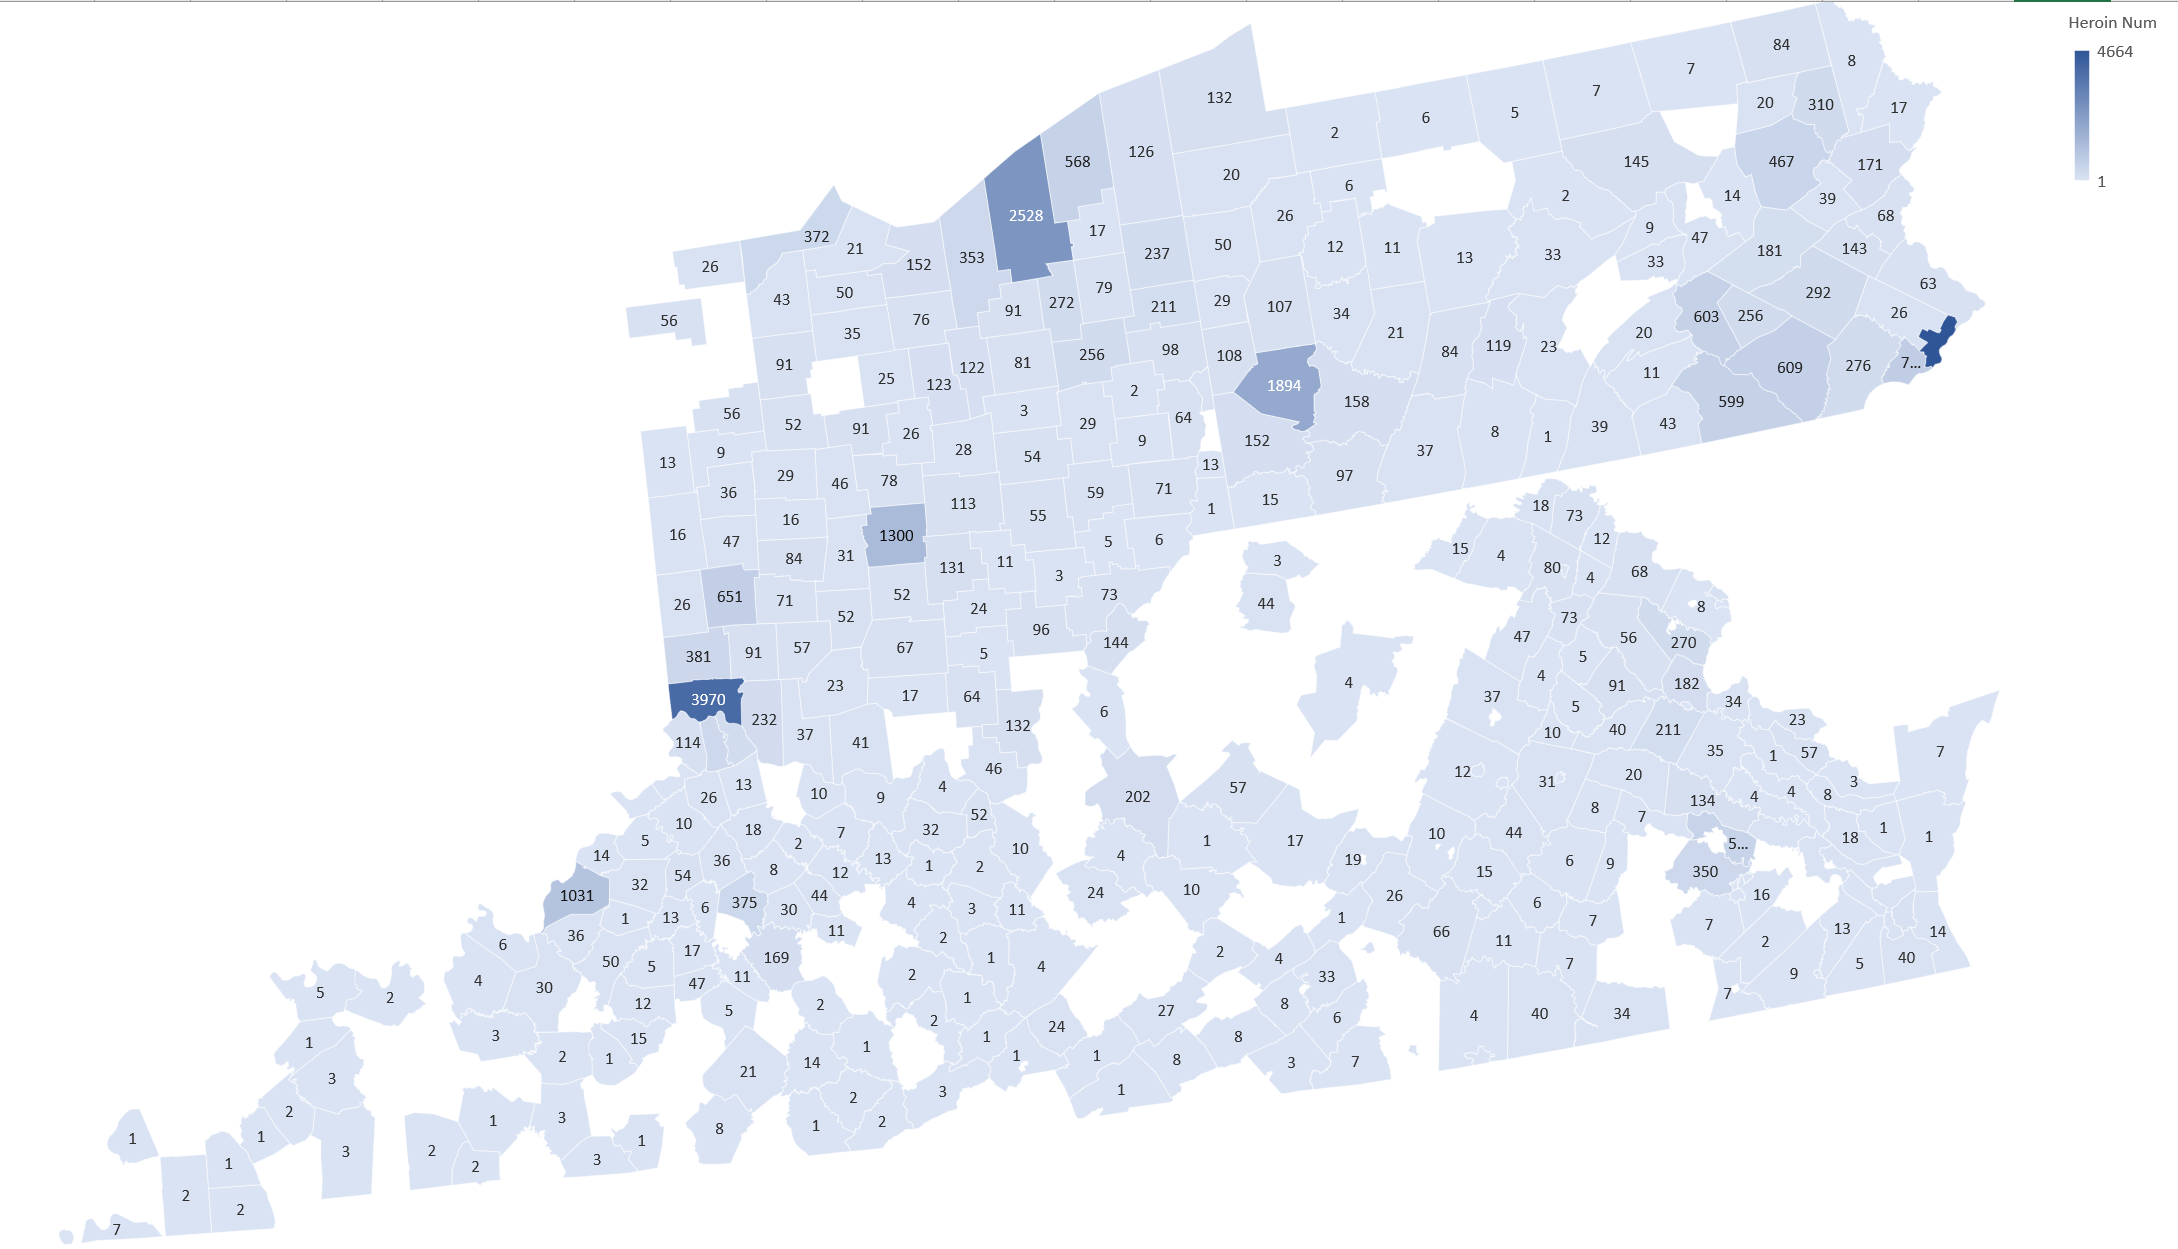
\includegraphics[width=\linewidth]{2017.png}
%      \caption{2017 Heroin}\label{H17}
%   \end{minipage}
% \end{figure}



% \begin{figure}[H]
%   \begin{minipage}{0.5\textwidth}
%      \centering
%      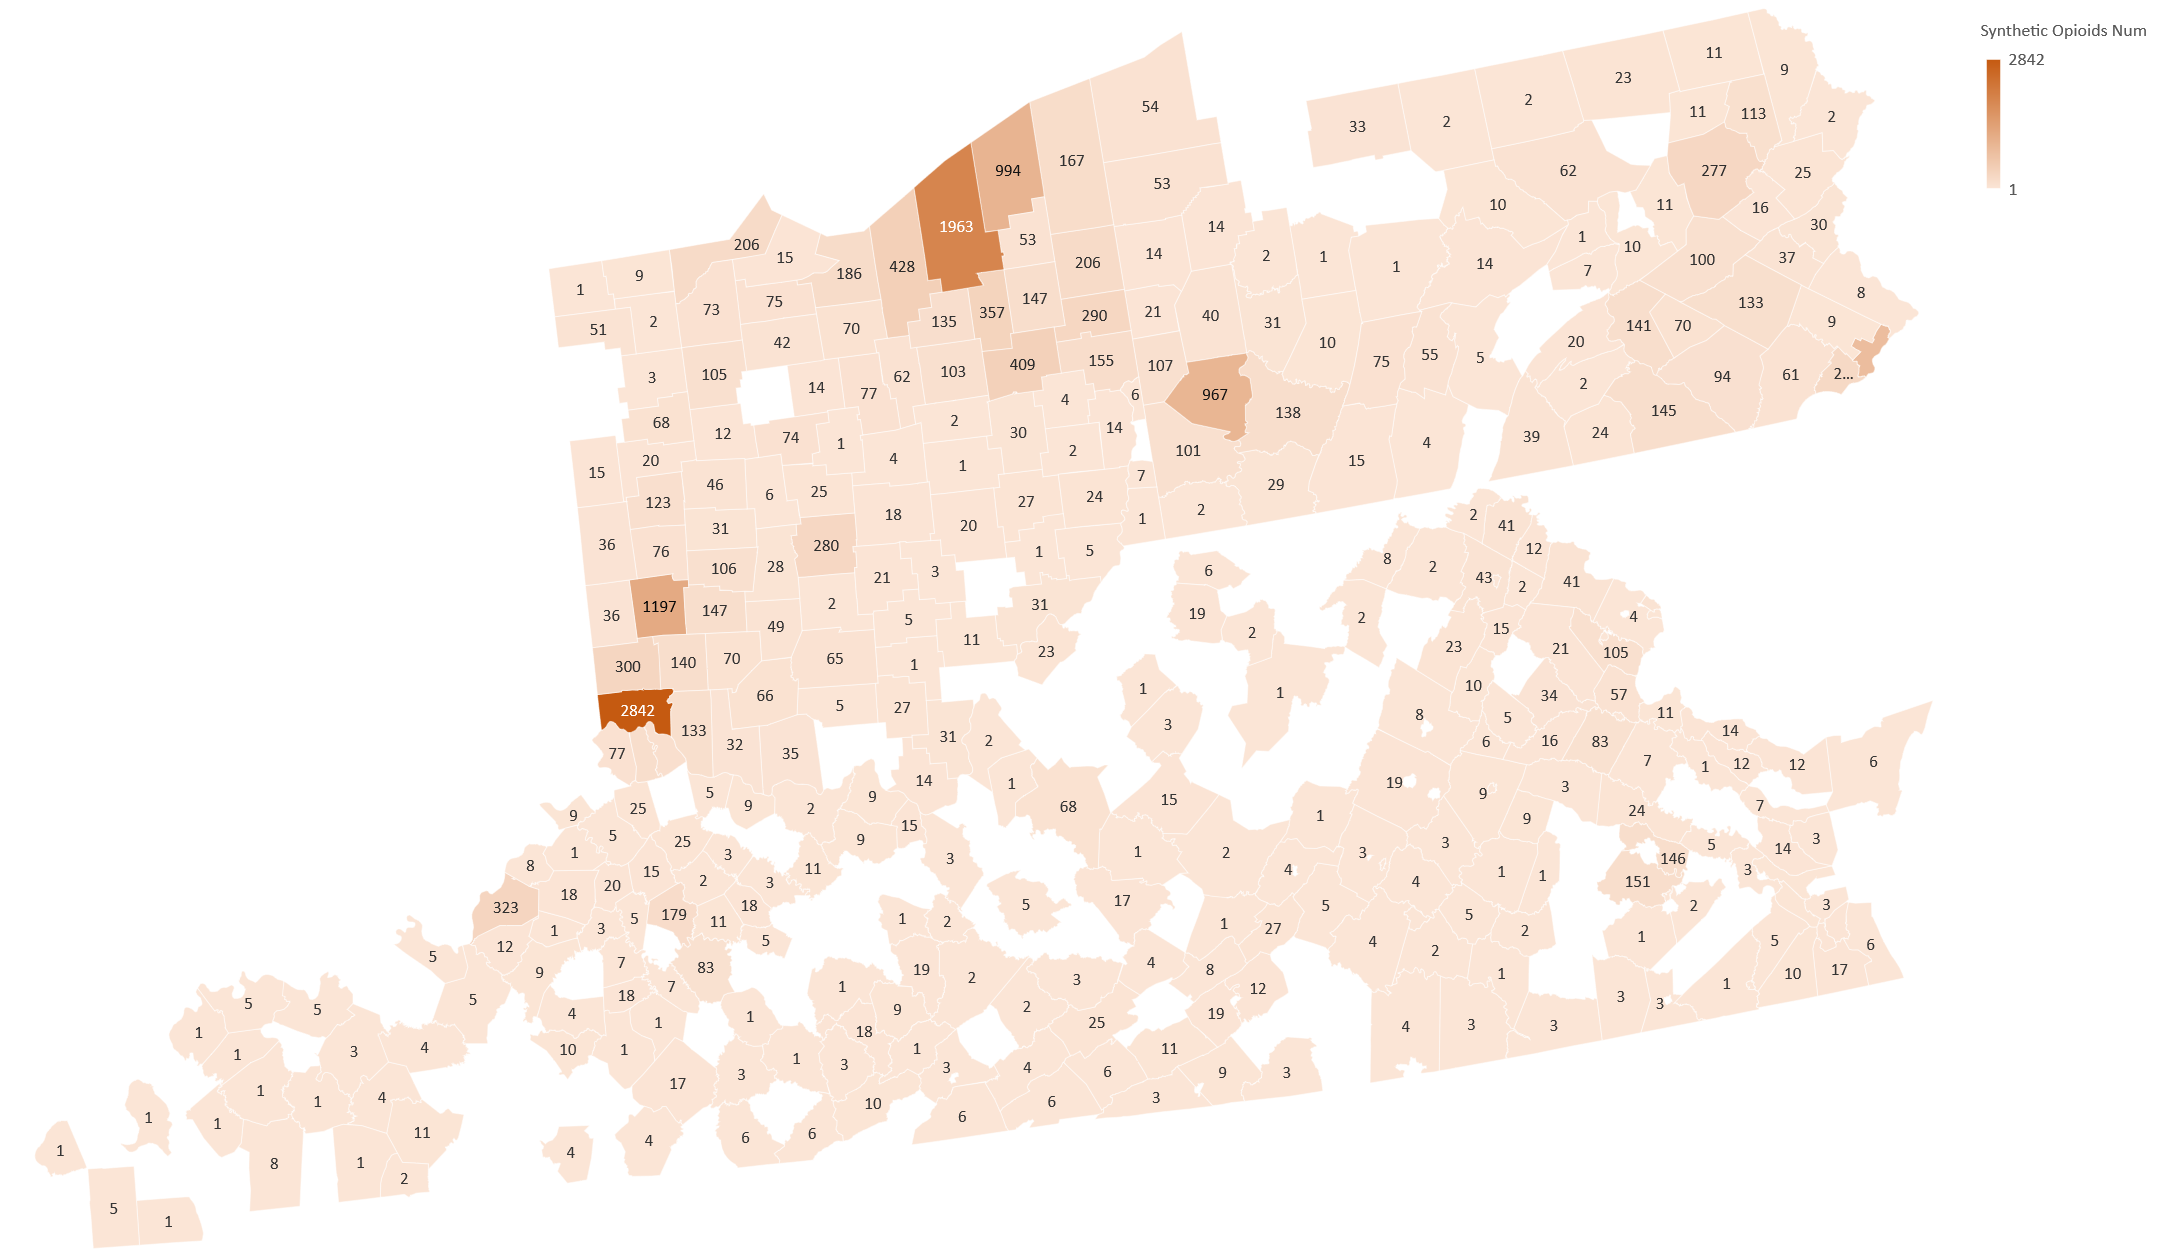
\includegraphics[width=\linewidth]{2016SYN.png}
%      \caption{2016 Synthetic}\label{S16}
%   \end{minipage}%\hfill
%   \begin{minipage}{0.5\textwidth}
%      \centering
%      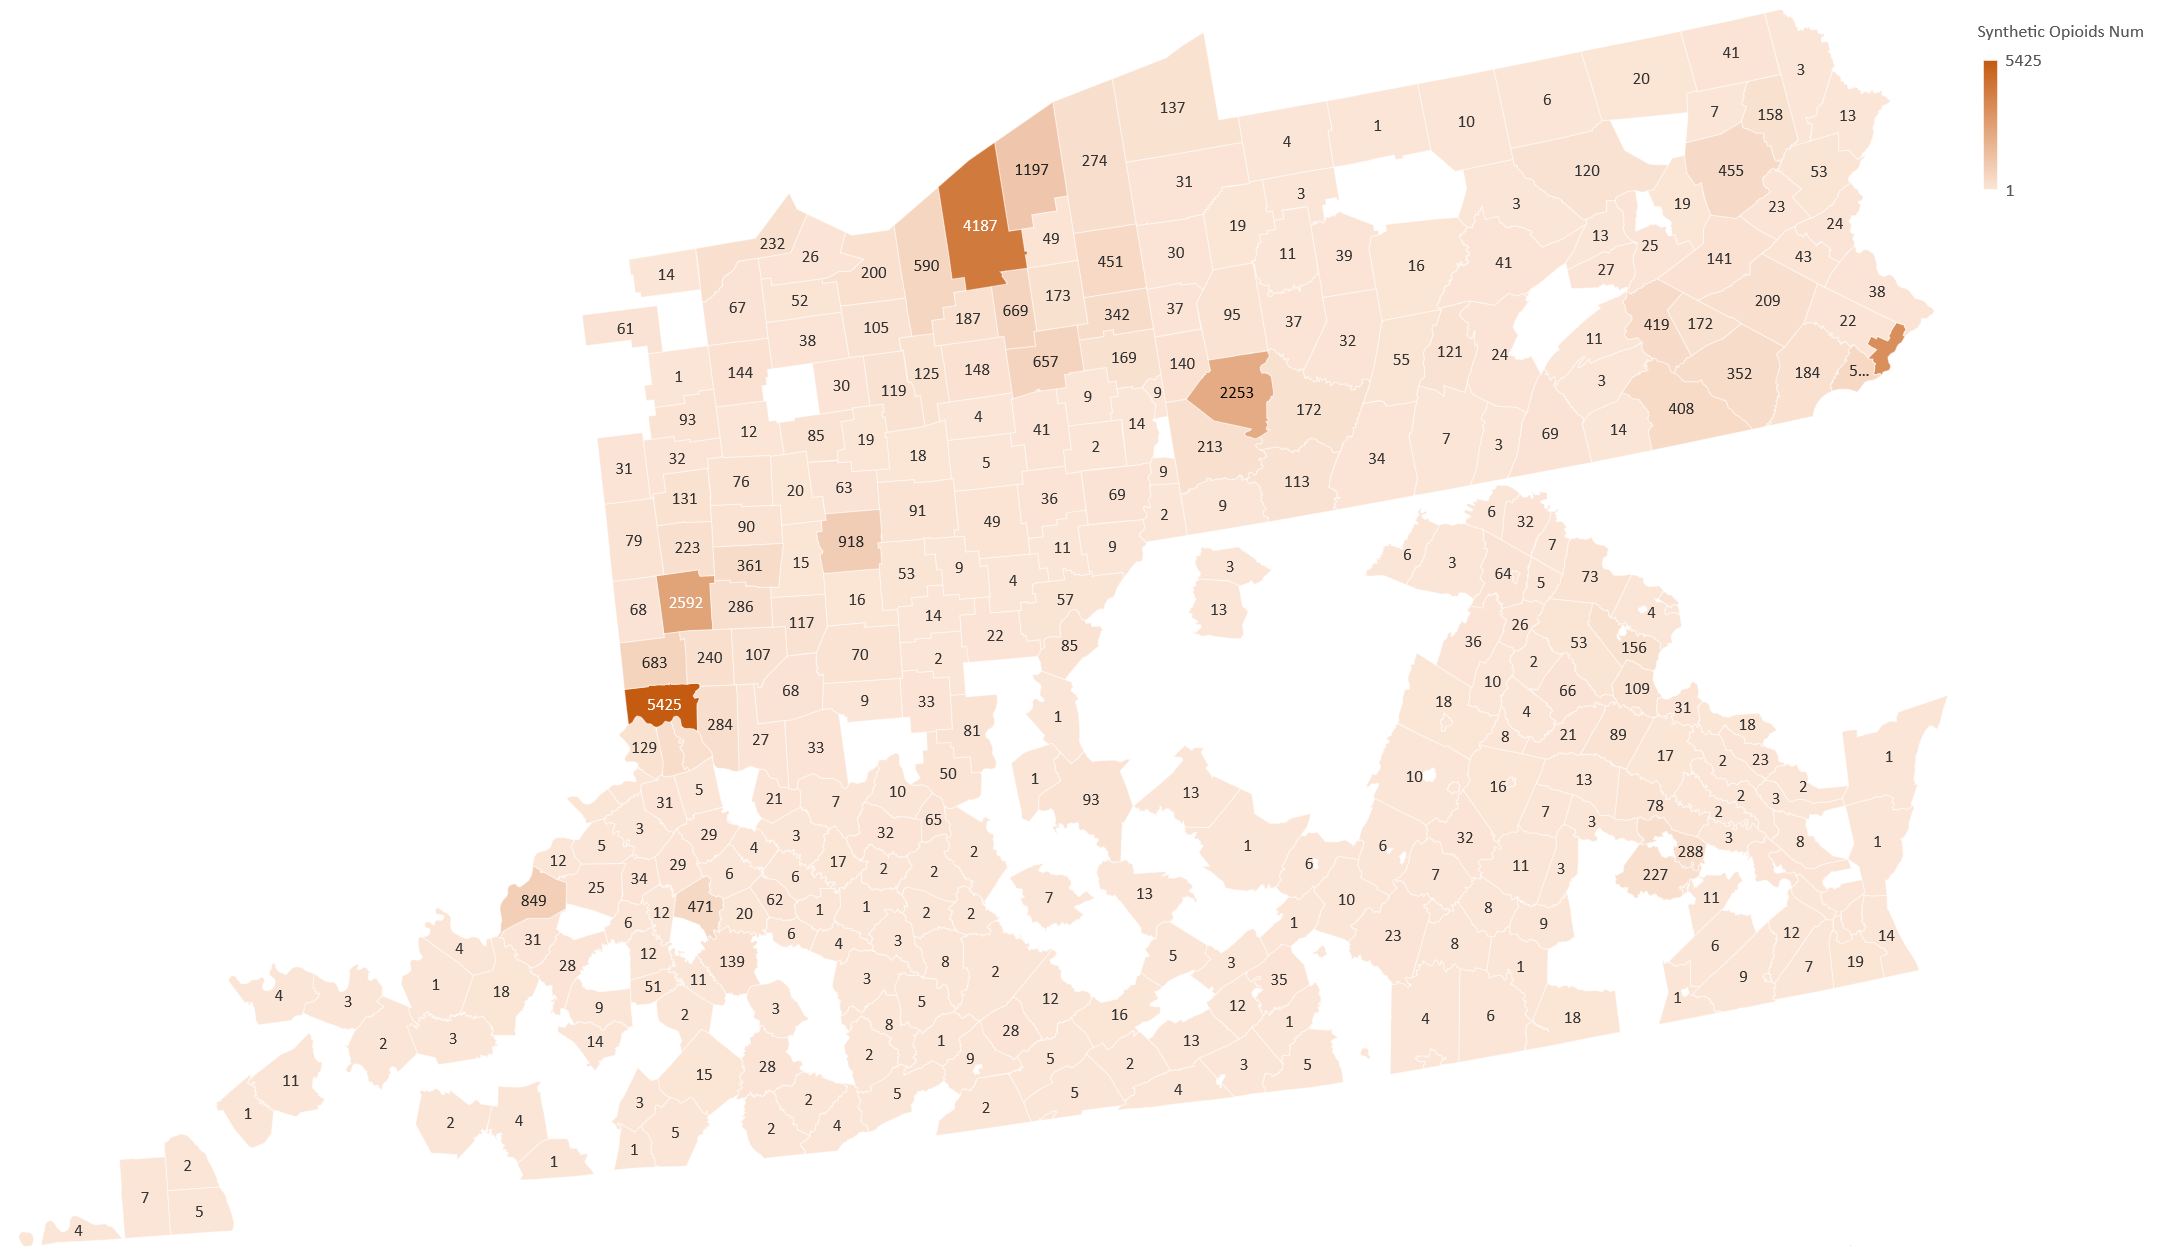
\includegraphics[width=\linewidth]{2017SYN.png}
%      \caption{2017 Synthetic}\label{S17}
%   \end{minipage}
% \end{figure}

%----------------------------------------------------------------
%---------------------END ADD IT BACK-----------------------------
%----------------------------------------------------------------

\subsection{Cellular Automaton (CA) Model Framework}

%In this model, we assume a constant size of population with recruitment and non-illicit-related death rate at time $t$ given by $\mu$. We separated the total population into several groups, including susceptible individuals, light and heavy drug users, people with mentally illness because of drugs, and detected illicit drug users.

%\begin{align}
%    N(t) = S(t) + I(t) + I_a(t) + M(t) + R(t),
%\end{align}
%~\\
%Then we assume that susceptible individuals acquire illicit drug use habits at rate \begin{align}
%    \lambda = \beta (I + \kappa I_a)
%\end{align}
%~\\
%The model then takes the form \begin{align}
%\begin{split}
%    \frac{dS}{dt} &= \mu - \lambda S - \mu S, \\
%    \frac{dI}{dt} &= \lambda S - (\alpha + \gamma + \sigma + \mu + \psi)I, \\
%    \frac{dI_a}{dt} &= \alpha I - (\rho + \phi + \mu + d)I_a, \\
%    \frac{dM}{dt} &= \sigma I + \phi I_a - (\epsilon + \mu + \delta)M, \\
%    \frac{dR}{dt} &= \gamma I + \rho I_a + \epsilon M - (\mu + \omega)R
%\end{split}
%\end{align}
%~\\
%Put equations (3) in the closed set, we will have \begin{align}
%    \Omega = \{(S, I, I_a, M, R) \in %\mathbb{R}^5_+ : 0 \le N \le 1\},
%\end{align}
%~\\
%where $\Omega$ is positively invariant with respect the the above equations (2).

For the purpose of our model, we decide to use a 2-D cellular automaton system. In spite of the simplicity of their structure, the Cellular Automaton(CA) we use can perform quite complex trend and involvement of the drug crisis that we are going to analyze if given enough constraints and parameters.\\
A cellular automaton (referred as CA in the following text) is characterized by the following five properties:
\begin{enumerate}
\item the number of spatial dimensions ($n$);
\item the width of each dimension ($w$), $w_j$ is the width of the $j$th dimension where $j = 1,2,...,n$;
\item the width of the neighborhood of each cell $(d)$. $d_j$ is the width of the neighborhood of the $j$th dimension;
\item the local status of each of the CA cells;
\item the CA rule, which is an arbitrary function called $F$.
\end{enumerate}
Notice that the change of state of a specific cell from time $t$ to $t+1$ is computed according to $F$. $F$ is a function of the state of itself as well as all the neighborhood cells at time $t$. 

Our CA model is a 2 dimensional grid where the width of the two sides are taken to be equal, namely $w_1 = w_2$. Each cell in the grid represents a county according to the geographic information on map such that the location and neighborhood information is well-preserved in this grid. Although not accurate and non-realistic, for this specific problem, we are restricting the inter-county communication only to the neighborhood counties, that is, a county can only be influenced by its 8 neighbors, namely on the top, left, right, bottom, top left, top right, bottom left and bottom right. We will discuss the impact of global communication in later sections.

At the initial time, where the time $t$ is at 2017, we assign a initial state to each of the cell in the grid according to a specific local rule. This rule is defined as following:

The state $C_{i,j}^t$ of the $(i,j)$ CA cell at time $t$ is
\begin{equation}
   C^t_{i,j} = \{S_{i,j}^t,\text{ INF}^t_{i,j}\},
   \label{state}
\end{equation}
where $\text{INF}^t_{i,j}$ is a `infectious flag' with only binary values 0 and 1. The value of the flag indicates whether there are drug reports from this state at time $t$ or not. If $\text{INF}^t_{i,j} = 1$, then the $(i,j)$ cell is a drug infected county.[2]

The transition of the state of each cell each time step is done according to the following function:
\begin{align}
\begin{split}
    S_{i,j}^{t+1} &= (1 + (\rho \cdot [S_{i,j}^t > \kappa]))\cdot S_{i,j}^t \\
    &+ k\cdot (S_{i-1,j}^t + S_{i,j-1}^t + S_{i,j+1}^t + S^t_{i+1,j})\\
    &+ l \cdot (S_{i-1,j-1}^t + S_{i+1,j-1}^t + S_{i-1,j+1}^t + S^t_{i+1,j+1}).
\end{split}
\label{CArule}
\end{align}
The state of the cell $(i,j)$ at time $t+1$ depends on both within the county and the state of all the 8 neighbors around it as shown in Figure \ref{grids}. 

\begin{figure}[H]
    \centering
    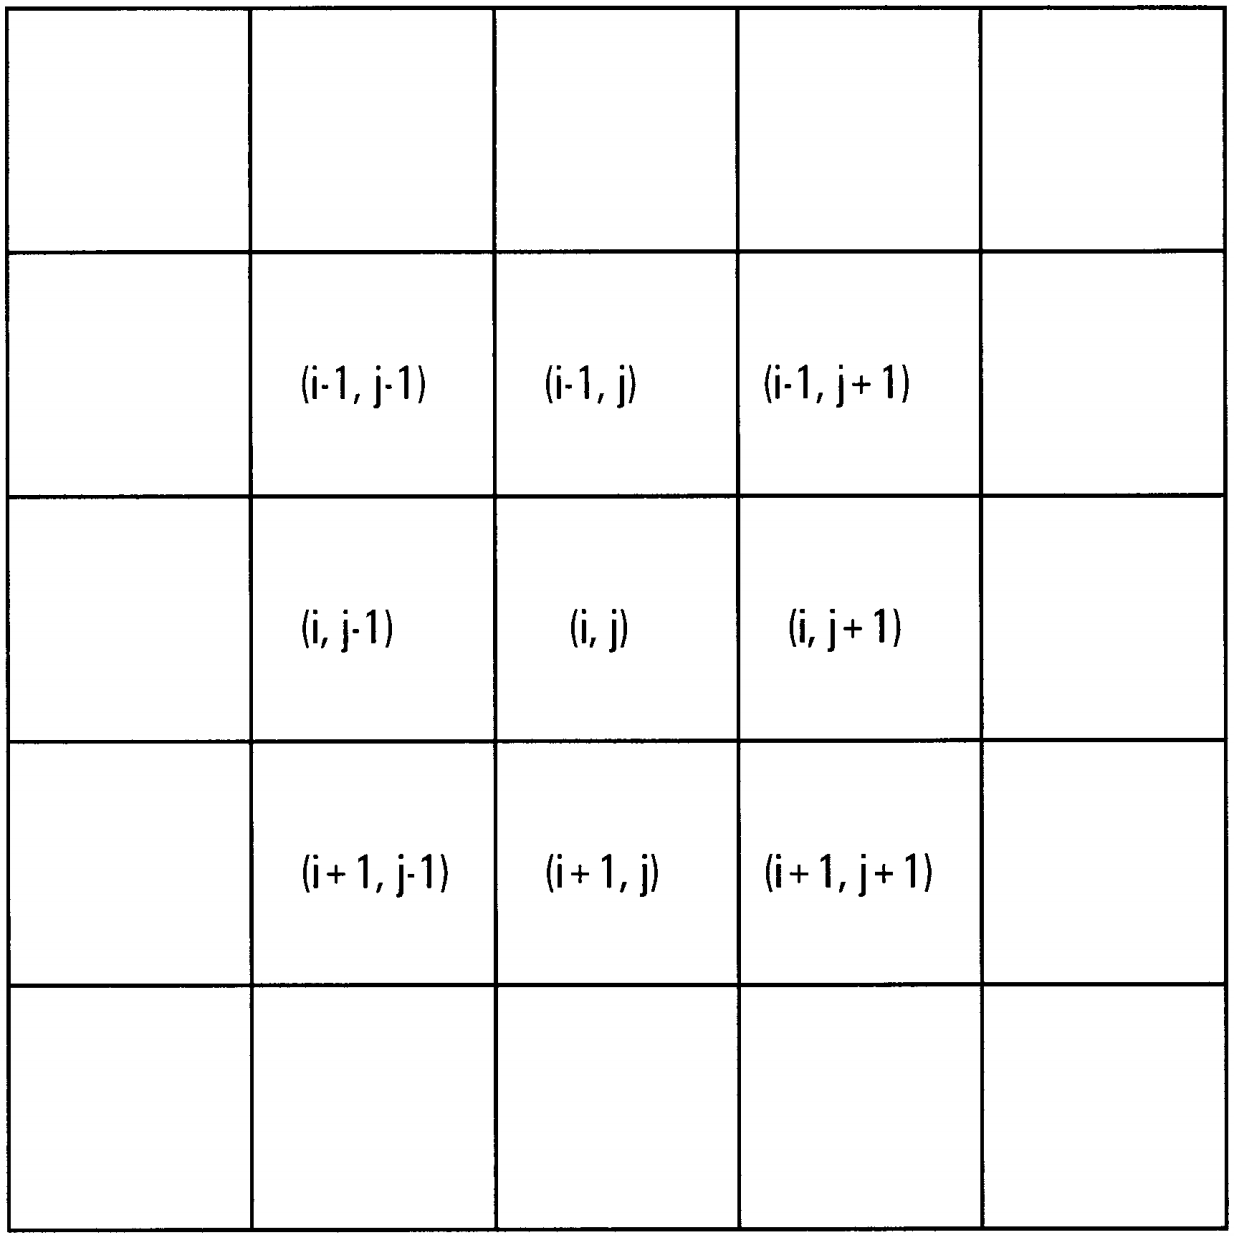
\includegraphics[width = 0.5\textwidth]{grids.png}
    \caption{Neighborhood cells of the $(i,j)$ cell}
    \label{grids}
\end{figure}

But the neighborhood influence is at a different rate since they have different boarder lengths. The effect of the adjacent neighbors, namely, $(i-1,j), (i+1,j), (i,j-1), (i,j+1)$ is multiplied by $k$ and the effect of the diagonal adjacent neighbors is multiplied by $l$. Notice that the cells with common sides have more connection with $(i,j)$, while the other four cells which are on the corners would have less connections and thus have less influence on the central one. Therefore, it is always the case that $k > l$.

On the other hand, there are influence within each county, too. Apart from the influence from the neighbors, the size of drug users would increase within the county itself if no severe regulation is posted. Therefore, $\rho$ is the self increasing rate of a county if the drug community in that county is larger than some threshold $\kappa$. 

\subsection{CA on Data}


%%%%%%%%%------------------------
%--------------------------------------
%-----------------------------------
%--------End of section 3-----------------
%------------------------------------
%--------------------------------------
%---------------------------------------

\newpage % delete this code
\section{}

\newpage
\section{Strengths and Weaknesses}
\subsection{Strengths}
\begin{itemize}
    \item 
\end{itemize}

\subsection{Weaknesses}
\begin{itemize}
    \item As we convert the actual map data to Cellular Automaton, we neglect counties with small reports number and relatively very small areas. Since both areas and numbers of reports are fairly small, neglecting them is less likely to cause serious errors on our output.\\
    However, since we fit each county into small grids, each of which has eight neighbors, the distance factor and neighbor information might  deviates the modelling output from the actual data. This chiefly happens when the area of the county is small in comparison to most of its neighbors. 
\end{itemize}
% - - - - - - - - - - - END Model Design - - - - - - - - - - -



% - - - - - - - - - - - Model Solution - - - - - - - - -

% labels allow you to cross-reference a section later in the document, without having to remember its number
%  - - - - - - - - - - - - - - - - - - - - - - - - - - - - - -
% Delete existing text when writing your own report.


 

% - - - - - - - - - - - END Discussion - - - - - - - - - - -



% - - - - - - - - - - - References - - - - - - - - -
% [1] http://www.comap-math.com/mcm/2019\_MCM-ICM\_Problems.zip


% - - - - - - - - - - - END References - - - - - - - - - - -




% = = = = = = = = = = = = = = = = = = = = = = = = = = = = = = 
%				END YOUR DOCUMENT - did you proofread?
% = = = = = = = = = = = = = = = = = = = = = = = = = = = = = = 
\end{document} % End of document. Nothing after this line will appear in .pdf
% = = = = = = = = = = = = = = = = = = = = = = = = = = = = = = 